\documentclass{article}
\usepackage[utf8]{inputenc}
\usepackage{listings}
\usepackage{CJKutf8}
\usepackage{amsmath}
\usepackage{amssymb}
\usepackage{graphicx}
\usepackage{algorithm}
\usepackage{algpseudocode}
\usepackage{float}
\usepackage{tikz}
\usepackage{url}
\usetikzlibrary{trees}
\usetikzlibrary{arrows}
\usepackage{subcaption}

\title{DSA HW4}
\author{B09901142 EE3 呂睿超}
\date{June 2023}

\usepackage{xcolor}

\definecolor{codegreen}{rgb}{0,0.6,0}
\definecolor{codegray}{rgb}{0.5,0.5,0.5}
\definecolor{codepurple}{rgb}{0.58,0,0.82}
\definecolor{backcolour}{rgb}{0.95,0.95,0.92}

\tikzset{
  treenode/.style = {align=center, inner sep=0pt, text centered,
    font=\sffamily},
  arn_n/.style = {treenode, circle, white, font=\sffamily\bfseries, draw=black,
    fill=black, text width=1.5em},% arbre rouge noir, noeud noir
  arn_r/.style = {treenode, circle, red, draw=red, 
    text width=1.5em, very thick},% arbre rouge noir, noeud rouge
  arn_x/.style = {treenode, rectangle, draw=black,
    minimum width=0.5em, minimum height=0.5em}% arbre rouge noir, nil
}
\lstdefinestyle{mystyle}{
    backgroundcolor=\color{backcolour},   
    commentstyle=\color{codegreen},
    keywordstyle=\color{magenta},
    numberstyle=\tiny\color{codegray},
    stringstyle=\color{codepurple},
    basicstyle=\ttfamily\footnotesize,
    breakatwhitespace=false,         
    breaklines=true,                 
    captionpos=b,                    
    keepspaces=true,                 
    numbers=left,                    
    numbersep=5pt,                  
    showspaces=false,                
    showstringspaces=false,
    showtabs=false,                  
    tabsize=2
}

\lstset{style=mystyle}

\begin{document}
\begin{CJK*}{UTF8}{bsmi}
\maketitle

\section{Problem 1 - Raffle Tickets}
\textbf{All problems in this section are done all by myself}

\begin{enumerate}

    \item \begin{enumerate}

    \begin{figure}[H]
        \centering
    \begin{subfigure}{.55\textwidth}
      \centering
      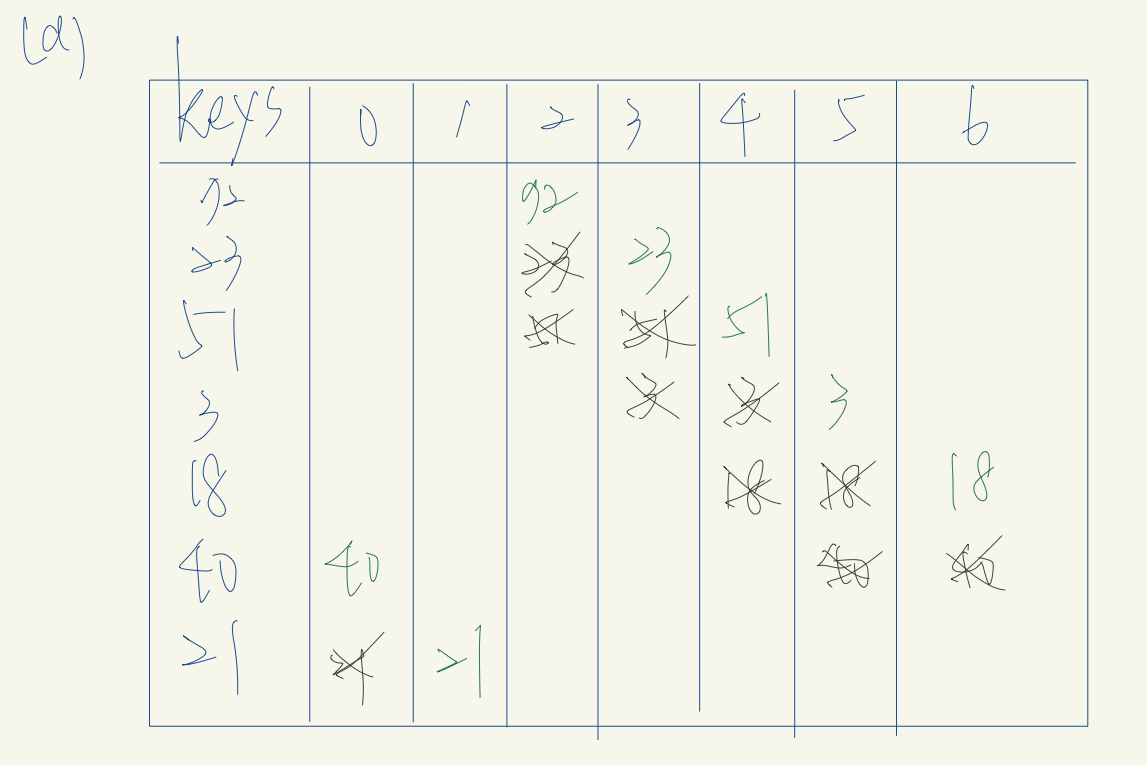
\includegraphics[width=1\linewidth]{IMG_0318.jpg}
      \caption{Linear Probing}
      \label{fig:sub1}
    \end{subfigure}%
    \begin{subfigure}{.5\textwidth}
      \centering
      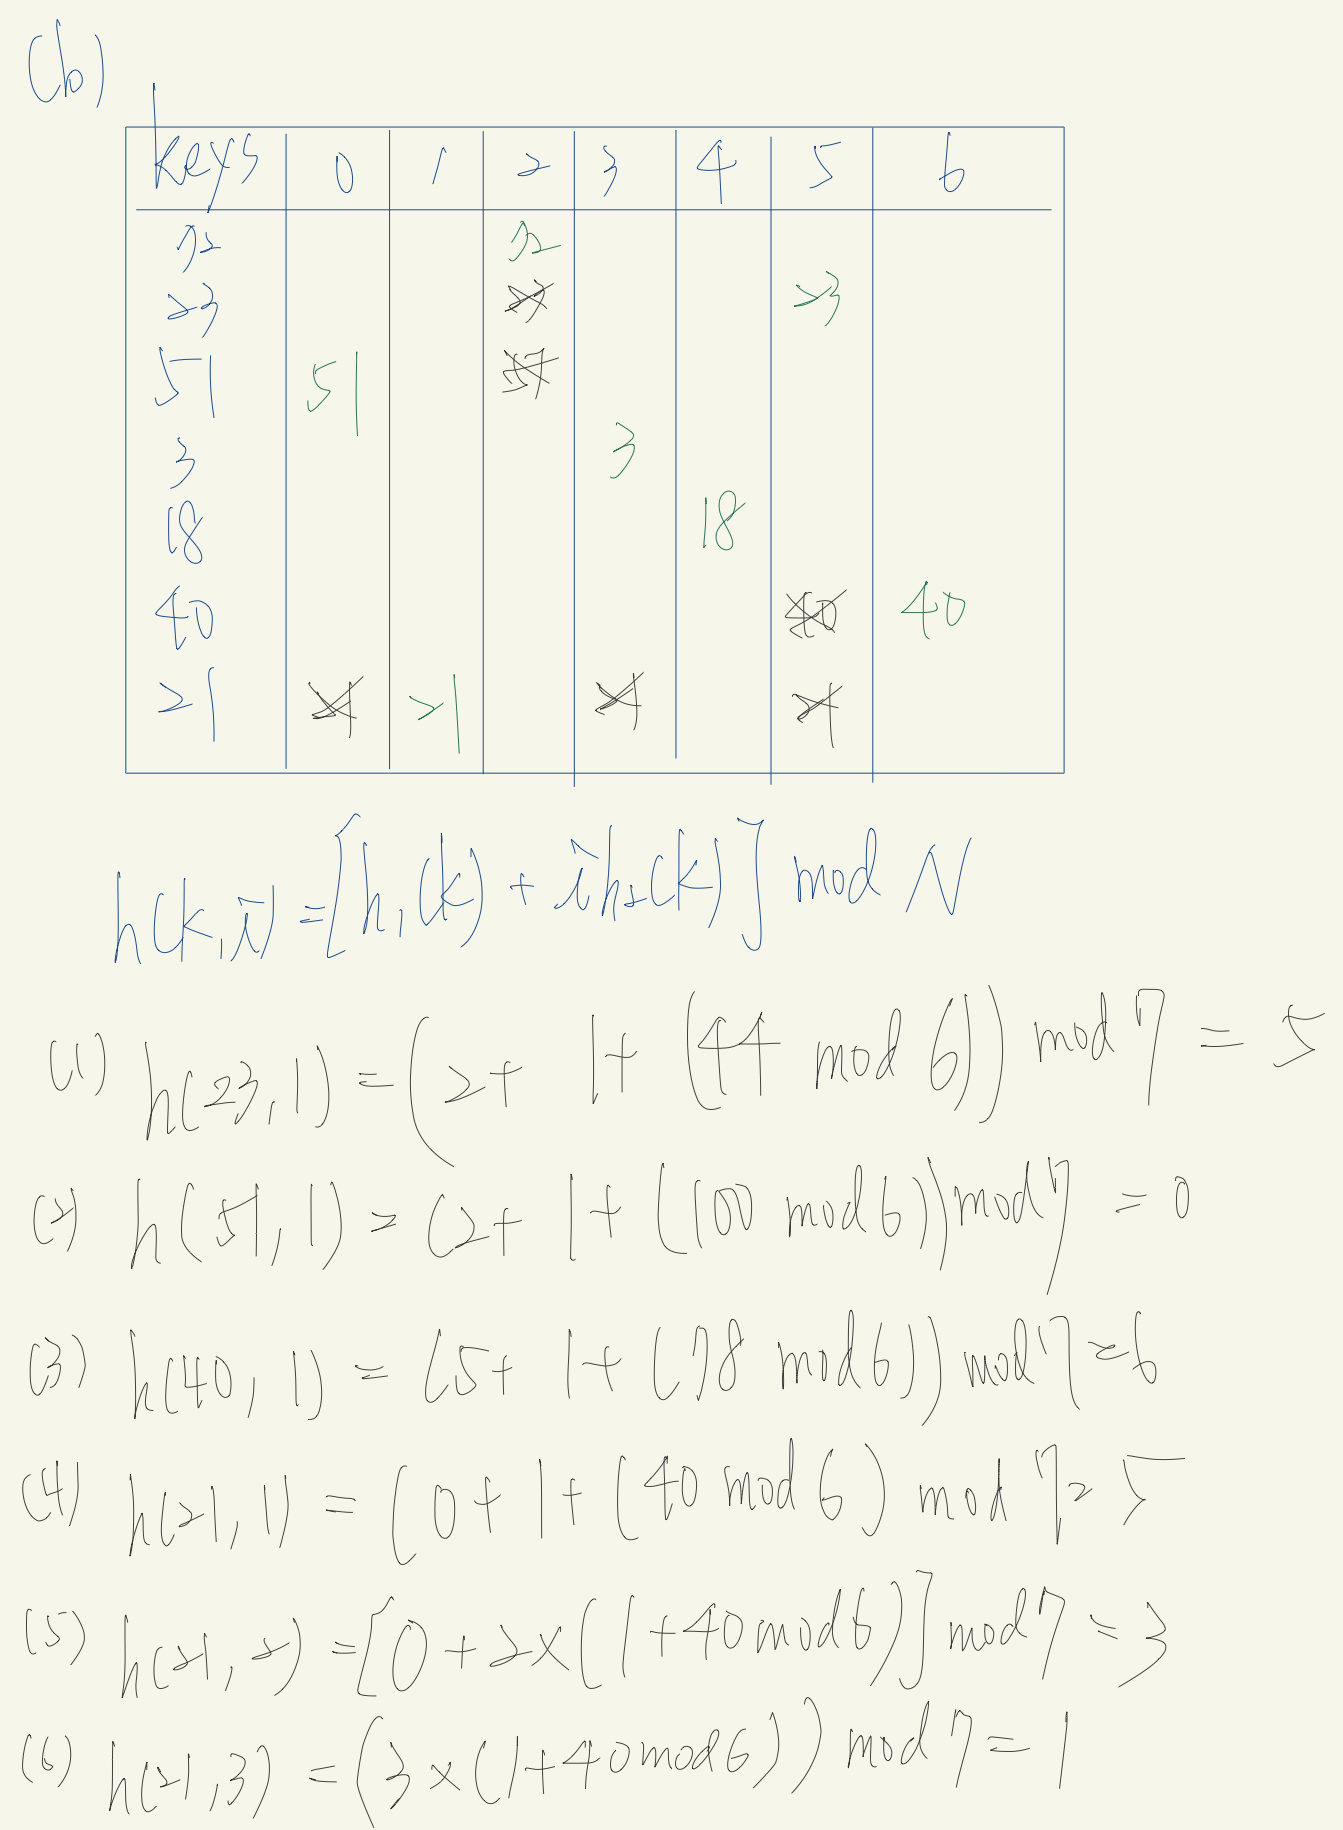
\includegraphics[width=1.2\linewidth]{IMG_0319.jpg}
      \caption{Double Hashing}
      \label{fig:sub2}
    \end{subfigure}
    \caption{Figures for Problem 1-1}
    \label{fig:test}
    \end{figure}
    \item For linear probing, I follow the hash function $h_1(x) = 8n mod(7)$ to do the first attempt to insert. If it fails, I cross out the attempt and follow the linear probing sequence to find available slots.
    \item Similar for double hashing, I cross out the first attempts of each insert and wrote the calculations of each double hashing for each $i \neq 0, h(k,i) = (h_1(k)+i*h_2(k) mod N)$. 
    \end{enumerate}
    \item \begin{enumerate}
        \item First, we can use the method in Rabin-Karp to hash a name in O(L).
        \item For the rotations, we can use a similar version of the update method in Rabin-Karp $(T_n$ update to $T_{n+1})$. 
        \item Assume the original name is T[\textbf{1},..,n], we can calculate h(T[\textbf{2},..,n,1]) by $h(T[\textbf{2},..,n,1]) = (h(T[\textbf{1},..,n] - h(T[1])*d^{n-1}) * d + h(T[2])*d^{n-1}) + h(T[1])$ (note that  $h(\textbf{T[2]})*d^{n-1} = h(T[2])*d^{n-1} + h(T[2])*d^{n-1}$ because d for upper and lower alphabets are same) (Note that the bolded characters represent that they are upper case letters.)
        \item The operation mentioned above cost $O(1)$ and there are L-1 rotations. Therefore, overall time complexity is $O(L)$
    \end{enumerate}
    \item \begin{enumerate}
        \item We can observe that each draw is independent since the tickets are returned to the pool after the draw.
        \item Therefore we can calculate that the probability of any two draws to have identical result is $\frac{1}{840}$ or $\frac{1}{840^2} *840$. (Or we can consider the situation as the probability of the collision of two values of uniform hashing with 840 slots.)
        \item Since there are 30 prizes (i.e. 30 draws) with probability of each pair of "draw collision" = $\frac{1}{840}$, the overall probability is $\frac{(30,2)}{840} \approx 0.517$ which isn't a coincidence.
    \end{enumerate}    
    \item \begin{enumerate}
        \item For question (a), the probability of each $s_i$ occurring spurious hit is $\frac{1}{p}$. Therefore, the total probability of occurring spurious hit is $\frac{n}{p} \approx 0.0001$.
        \item For question (b), we can calculate the probability in the complement way. Consider if n different strings can be perfectly hashed into n different hash value. The probability of achieving this is 
        \[ \frac{\textbf{P}(P,n)}{P^n} \approx 0.00067\]
        Which means that the probability of occurring spurious hit is 1- 0.00067.
        \item Following the previous two points, we can conclude that the the probability of occurring spurious hit is way larger in (b) than in (a), which satisfies the question.
    \end{enumerate}
\end{enumerate}

\section{Problem 2 - README}
\textbf{All problems in this section are done all by myself}
\begin{enumerate}
    \item \begin{enumerate}
        \item The maximum ratio of good ones to bad ones is 2
        \item Consider a full tree since the ratio would reach maximum. Following the rules of RB tree, there are no consecutive red node. Therefore, to reach the maximum number of red nodes, we need to put red nodes on the level with more nodes.
        \item In conclusion, we can consider a full tree containing odd levels (height is an odd number) with black nodes and even levels with red nodes. 
        \item The example of the RB tree with 15 nodes and reaching maximum red nodes is as the following figure.
        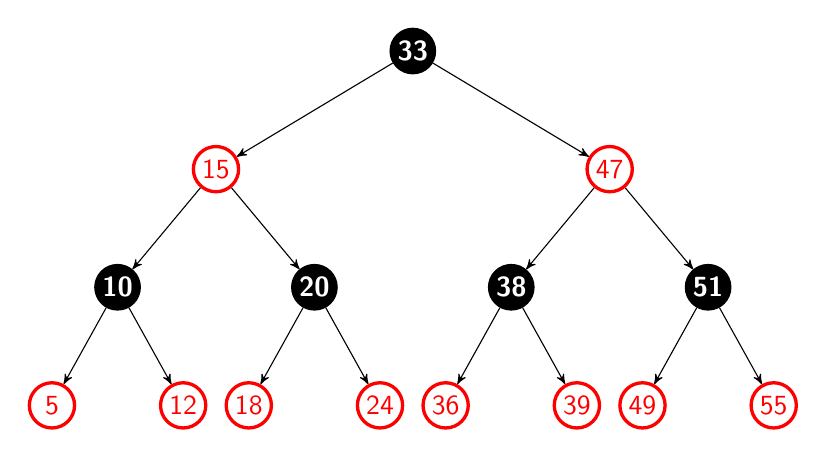
\begin{tikzpicture}[->,>=stealth',level/.style={sibling distance = 5cm/#1,
  level distance = 1.5cm}] [h]
\node [arn_n] {33}
    child{ node [arn_r] {15} 
            child{ node [arn_n] {10} 
            	child{ node [arn_r] {5} } 
							child{ node [arn_r] {12}}
            }
            child{ node [arn_n] {20}
							child{ node [arn_r] {18}}
							child{ node [arn_r] {24}}
            }                            
    }
    child{ node [arn_r] {47}
            child{ node [arn_n] {38} 
							child{ node [arn_r] {36}}
							child{ node [arn_r] {39}}
            }
            child{ node [arn_n] {51}
							child{ node [arn_r] {49}}
							child{ node [arn_r] {55}}
            }
		}
; 
\end{tikzpicture}
    \end{enumerate}
    
    \item  
    \begin{enumerate}
        \item The main idea is to add an information of its left subtree size to each node.We can utilize the postorder traverse to obtain the size of each left subtree. Also, in order to obtain the left subtree size, we also need to add the whole subtree size(left + right)
        \item When doing postorder traverse, each leaf node is updated as subtree size = left subtree size
         = 1 
        \item When updating a parent node, we update its subtree size = left child's subtree size + right child's subtree size. Also, we update its left subtree size = left child's subtree size.
        \item The implementation can query k-th smallest element in O($log(n)$). Starting from the root, we use a similar approach of searching in BST or RB tree. Starting from the root, if k $>$ \textbf{current node's left subtree size - 1}, we move to the right child, else if k $<$ \textbf{parent node's left subtree size + current node's left subtree size - 1} we move to the left child, else (equal situation), we output the current nodes $d_i$
        \item Note that in the previous point, every time we move to the right child, we need to record the current considering \textbf{parent node's left subtree size + current node's left subtree size - 1}, which we can denote as k' in order to move on to the next right path.(A more concise way is that we can change k to k-parent node's left subtree size when we move right)
    \end{enumerate}
 
        
    \item  \begin{enumerate}
        \item The insertion and deletion are all based on a rule. When we move left, we change the current node's left subtree size and subtree size.
        \item For insertion, it is similar with  BST or RB tree insertion. When we move to the left, we change the \textbf{current node's left subtree size} to \textbf{current node's left subtree size + 1}. Identical change is done with the subtree size. 
        \item When we insert the new node as a leaf, each leaf node is updated as subtree size = left subtree size = 1 
        \item The change in rotaion: \begin{enumerate}
            \item left rotation : We use B as A's right child as an example. After left rotation, the data needed to update is \textbf{B's left subtree size += A's left subtree size}, 
            \item right rotation: We use B as A's left child as an example \textbf{A's left subtree size -= B's left subtree size}.
        \end{enumerate}
        \item For deletion, similar with insertion : when we move to the left, we change the \textbf{current node's left subtree size} to \textbf{current node's left subtree size - 1}. Identical change is done with the subtree size. 
        \item The change in rotation is the same as the case in insertion
        \item The case that we replace the node with its predeceesor, just inherit the updated data(the data that has minus one) from the deleted node.
    \end{enumerate}

    
    \item \begin{enumerate}
        \item The basic conecept is similar with the previous question, but now we need to add the information of the left subtree sum and "whole" subtree sum. (In order to keep concise, I would ignore some repetitive parts)
        \item For insertion, we now add update the left subtree sum and subtree sum by adding $z_i$. We update the leaf node's left subtree sum and subtree sum as $z_i$
        \item Change in rotation is similar with the case in the previous problem but now we update left subtree sum and subtree sum,
        \item For deletion, it is similar and repetitive(We change plus to minus(just like in the previous problem) and we focus on left subtree sum and subtree sum rather than their size.
        \item All operations above is \textbf{added} to the original operation from the previous problem.(The original operation is still needed to be done)
        \item For query(Finding x), it is also similar with the case in the previous problem but we focus on the subtree sum rather than left subtree size(But we still need left subtree sum in order to decide whether to go left or right). When we finally found the node that the subtree sum is equal or "quite bigger" than E, we output the current node's \textbf{subtree size}. 
    \end{enumerate} 
     
    
\end{enumerate}



\end{CJK*}
\end{document}
